\begin{topic}{Electronic Mail}

\textbf{User Agents}

A mail reader. 
Composing, editing, reading.
Emails are temporarily stored on the client.

\textbf{Mail Servers}

Mailbox for each user which stores incoming emails

Message queue of outgoing emails

\end{topic}

\begin{topic}{SMTP}
Uses TCP to send emails on port 25.

Direct transporation - sending server to receiving server

Three phases of transfer
\begin{enumerate}
	\item handshaking (greeting)
	\item transfer of messages
	\item closure
\end{enumerate}

SMTP is a persistent connection and requires 7-bit ascii messages.
\end{topic}

\begin{topic}{SMTP Transaction}
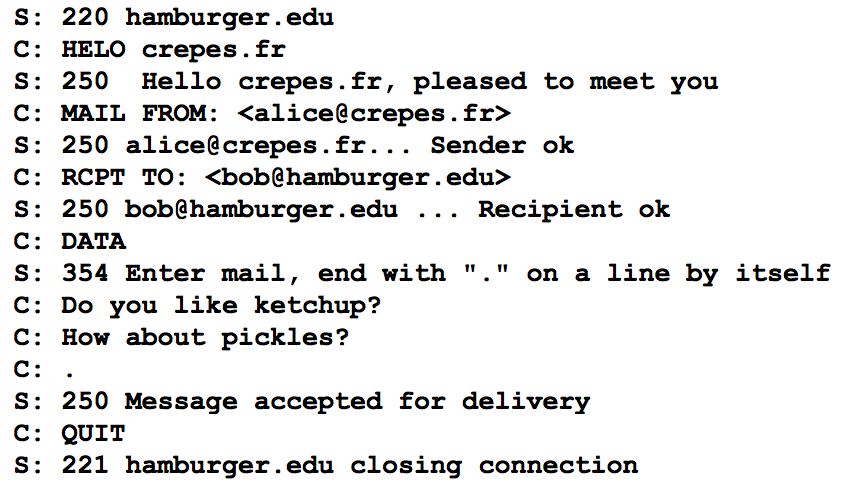
\includegraphics[scale=0.35]{coms3200/images/smtp}
\end{topic}

\begin{topic}{Mail Message Format}
Mail messages consist of a \textbf{header} containing To, From, Subject, etc fields.

Also contains a \textbf{Body} section in ASCII characters only.
\end{topic}

\begin{topic}{POP Protocol}
\begin{multicols}{2}
\textbf{Post Office Protocol} [RFC 1939]: authorization and download

Protocol has two phases: \textbf{authentication} and \textbf{transaction}.

\textbf{Commands:} user, pass, list, retr, dele, quit

\textbf{Responses:} +OK, -ERR

\columnbreak

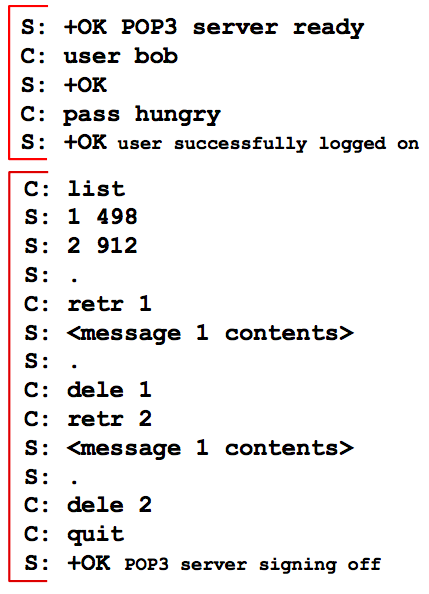
\includegraphics[scale=0.35]{coms3200/images/pop}
\end{multicols}
\end{topic}

\begin{topic}{IMAP Protocol}
\textbf{Internet Mail Access Protocol} [RFC 1730]

Keeps all messages on the \textbf{server}

Adds \textbf{folders} to store messages

Holds user states between sessions
\end{topic}
